\documentclass[dvipdfmx]{beamer}
%テーマの設定
\usetheme[numbering=fullbar]{focus}

%パッケージの設定
\usepackage{graphicx}
\usepackage{ulem}
\usepackage{pxjahyper}
\usepackage{hyperref}
\usepackage{tikz}
\usetikzlibrary{arrows.meta,positioning,shapes}
\usepackage{listings, jlisting}
\usepackage{listings-arduino, listings-html5, listings-javascript}
\usepackage{xcolor}

%色設定
\definecolor{identifier}{RGB}{225, 123, 52}       %#e17b34
\definecolor{comment}{RGB}{105, 130, 27}          %#69821b
\definecolor{keyword}{RGB}{170, 76, 143}          %#aa4c8f
\definecolor{string}{RGB}{39, 146, 195}           %#2792c3

%ソースコード設定
\lstset{
  basicstyle={\ttfamily\footnotesize},            % 基礎の文字のフォント設定
  identifierstyle={\color{identifier}},           % 変数名などのフォント設定
  commentstyle   ={\color{comment}},              % コメントのフォント設定
  keywordstyle   =[1]{\color{keyword}},           % 予約語のフォント設定
  stringstyle    ={\ttfamily\color{string}},      % 文字列のフォント設定
  tabsize=2
}

%フォント設定
\renewcommand{\kanjifamilydefault}{\gtdefault}

%メタ設定
\title{多言語プログラミング}
\subtitle{プログラミングにおける骨格}
\author[電研]{電気技術研究会}
\institute[NITNC]{NIT, Nara Collage}
\date[\today]{\today}
\titlegraphic{
  \begin{tikzpicture}[overlay, remember picture]
    \node[at=(current page.north east), anchor=north east]{
      
\includegraphics[height=0.15\textheight]{pic/Logo(2).png}
      \hspace{0.05\textwidth}
    };
  \end{tikzpicture}
}

\begin{document}

\begin{frame}[plain]
  \titlepage
\end{frame}

\section*{概要}
  \begin{frame}[plain,noframenumbering]
    \sectionpage
  \end{frame}
  \begin{frame}{講義目的と進め方}
    \begin{large}講義目的\end{large}
    \begin{itemize}
      \setlength{\itemsep}{5mm}
      \item \structure{多言語}にわたるプログラミングを\structure{独学する}術を身に付ける
      \item 基本的な\structure{用語}や\structure{技術}を学び \structure{活かせる力}を身に付ける
      \item マイコンやウェブなど \structure{広い範囲に適応できる}人材育成
    \end{itemize}
    \vfill
    \begin{large}進め方\end{large}
    \begin{itemize}
      \setlength{\itemsep}{5mm}
      \item 重要な\structure{章}ごとにまとめて講義
      \item 1日(\structure{2~3時間})\structure{1~2}章分を進めたい
      \item 各章ごとに\structure{演習}がある
    \end{itemize}
  \end{frame}

  \begin{frame}{カリキュラム}
    \begin{tikzpicture}
      [every node/.style={rounded corners,inner sep=5pt, minimum width=100pt,minimum height=35pt},
      pre-subj/.style={fill=blue!20},post-subj/.style={fill=black!20},overlay, remember picture]
      \node[pre-subj] (a) at (0.15\textwidth,0.375\textheight){\hyperlink{programming}{プログラミング}};
      \node[pre-subj,below=10pt of a] (b) {\hyperlink{hensu}{変数とデータ型}};
      \node[pre-subj,below=10pt of b] (c) {\hyperlink{enzan}{演算と演算子}};
      \node[pre-subj,below=10pt of c] (d) {\hyperlink{seigyo}{制御構文}};
      \node[pre-subj,below=10pt of d] (e) {\hyperlink{hairetsu}{配列}};
      \node[pre-subj,right=10pt of e] (f) {\hyperlink{object}{オブジェクト}};
      \node[pre-subj,above=10pt of f] (g) {\hyperlink{kansu}{関数}};
      \node[pre-subj,above=10pt of g] (h) {\hyperlink{pointa}{ポインタ}};
      \node[pre-subj,above=10pt of h] (i) {\hyperlink{objectbun}{オブジェクト構文}};
      \node[pre-subj,above=10pt of i] (j) {\hyperlink{computer}{コンピュータ基礎}};
      \node[pre-subj,right=10pt of j] (k) {\hyperlink{micom}{マイコン}};
      \node[pre-subj,below=10pt of k] (l) {\hyperlink{iot}{IoT}};
      \node[pre-subj,below=10pt of l] (m) {\hyperlink{analys}{プログラム解析}};
      \node[pre-subj,below=10pt of m] (n) {\hyperlink{readability}{コードの可読性}};
      \node[pre-subj,below=10pt of n] (o) {\hyperlink{learn}{言語の学習法}};
      \foreach \x / \y in {a/b,b/c,c/d,d/e,e/f,f/g,g/h,h/i,i/j,j/k,k/l,l/m,m/n,n/o}{
        \draw[->,>={Stealth[round]},line width=.5mm] (\x) -- (\y);
      }
    \end{tikzpicture}
  \end{frame}

\section*{プログラミングとは}
  \begin{frame}[plain,noframenumbering]
    \label{programming}
    \sectionpage
  \end{frame}
  \begin{frame}{進度}
    \begin{tikzpicture}
      [every node/.style={rounded corners,inner sep=5pt, minimum width=100pt,minimum height=35pt},
      pre-subj/.style={fill=blue!20},now-subj/.style={white,fill=black!50!green},post-subj/.style={fill=black!20},overlay, remember picture]
      \node[now-subj] (a) at (0.15\textwidth,0.375\textheight){\hyperlink{programming}{プログラミング}};
      \node[pre-subj,below=10pt of a] (b) {\hyperlink{hensu}{変数とデータ型}};
      \node[pre-subj,below=10pt of b] (c) {\hyperlink{enzan}{演算と演算子}};
      \node[pre-subj,below=10pt of c] (d) {\hyperlink{seigyo}{制御構文}};
      \node[pre-subj,below=10pt of d] (e) {\hyperlink{hairetsu}{配列}};
      \node[pre-subj,right=10pt of e] (f) {\hyperlink{object}{オブジェクト}};
      \node[pre-subj,above=10pt of f] (g) {\hyperlink{kansu}{関数}};
      \node[pre-subj,above=10pt of g] (h) {\hyperlink{pointa}{ポインタ}};
      \node[pre-subj,above=10pt of h] (i) {\hyperlink{objectbun}{オブジェクト構文}};
      \node[pre-subj,above=10pt of i] (j) {\hyperlink{computer}{コンピュータ基礎}};
      \node[pre-subj,right=10pt of j] (k) {\hyperlink{micom}{マイコン}};
      \node[pre-subj,below=10pt of k] (l) {\hyperlink{iot}{IoT}};
      \node[pre-subj,below=10pt of l] (m) {\hyperlink{analys}{プログラム解析}};
      \node[pre-subj,below=10pt of m] (n) {\hyperlink{readability}{コードの可読性}};
      \node[pre-subj,below=10pt of n] (o) {\hyperlink{learn}{言語の学習法}};
      \foreach \x / \y in {a/b,b/c,c/d,d/e,e/f,f/g,g/h,h/i,i/j,j/k,k/l,l/m,m/n,n/o}{
        \draw[->,>={Stealth[round]},line width=.5mm] (\x) -- (\y);
      }
    \end{tikzpicture}
  \end{frame}

  \begin{frame}{プログラミングについて}
    \begin{large}プログラミングどんなもの?\end{large}
    \begin{itemize}
      \setlength{\itemsep}{3mm}
      \item プログラミングには様々な種類が存在\\ウェブ マイコン ゲーム...etc
      \item 大まかには2種類\\\structure{オブジェクト指向}と\structure{構造化プログラミング}(後述)
      \item \structure{骨格}は基本的に共通\\関数や変数など 基本的な\structure{骨格}がある
    \end{itemize}
    \vfill
    \begin{large}プログラミング言語\end{large}
    \begin{itemize}
      \setlength{\itemsep}{3mm}
      \item \structure{言語}は多数ある\par C, C++, C\#, JavaScript, VisualBasic, Python, \LaTeX
      \item 本教材では主に\structure{JavsScript}とArduinoによる\structure{C++}を使用
    \end{itemize}
  \end{frame}

  \begin{frame}[fragile]{基本的な骨格とは}
    \begin{columns}
      \begin{column}{0.6\textwidth}
        \begin{itemize}
          \item 冒頭で\structure{ライブラリ}の宣言
          \item \structure{メインループ}で処理\\UI等の場合では\structure{イベント}を処理
          \item \structure{サブルーチン(関数)}にて\\繰り返し処理
        \end{itemize}
        \centering
        \begin{minipage}{0.8\textwidth}
          \begin{exampleblock}{C言語の例}
            \begin{lstlisting}[language=C]
#include <stdio.h>

int main(void){
  printf('Hello World');
  return 0;
}    
            \end{lstlisting}
          \end{exampleblock}
        \end{minipage}
      \end{column}
      \begin{column}{0.4\textwidth}
        \begin{exampleblock}{Arduinoの例}
          \begin{lstlisting}[language=Arduino]
void setup(){
  pinMode(2, OUTPUT);
}
void loop(){
  digitalWrite(2, HIGH);
  delay(200);
  digitalWrite(2,LOW);
  delay(200);
}

          \end{lstlisting}
        \end{exampleblock}
      \end{column}
    \end{columns}
  \end{frame}

  \begin{frame}[fragile]{演習1:問題}{プログラミングとは}
    \begin{columns}
      \begin{column}{0.55\textwidth}
        \begin{large}JavaScript動作確認\end{large}
        \begin{enumerate}
          \setlength{\itemsep}{3mm}
          \item \structure{VSCode}の作業フォルダを作成
          \item {\color{string}'Hello World'}を表示させる
        \end{enumerate}
        \vspace{5mm}
        \begin{large}HTMLファイルへの埋め込み\end{large}
        \begin{itemize}
          \setlength{\itemsep}{3mm}
          \item \structure{html}ファイルの\structure{<script>}タグ内
          \item ディスプレイさせる関数\\
          \lstinline[language=javascript]|document.writeln('|{\color{string}\footnotesize 文字列 '}\lstinline[language=javascript]|)|
          \item 文末には\structure{;}をつける
          \item 文字列は\structure{’}か\structure{”}で囲う
        \end{itemize}
      \end{column}
      \begin{column}{0.45\textwidth}
        \begin{exampleblock}{htmlテンプレート}
          \begin{lstlisting}[language=html5,basicstyle=\tiny]
<html>
<head>
<meta
  http-equiv="Content-Type"
  content="text/html; charset=UTF-8">
<title>Hello,World!</title>
</head>
<body>
<pre>
<script type="text/javascript">
  // ここにスクリプトを記述
</script>
<noscript>
  JavaScriptが利用できません。
</noscript>
</pre>
</body>
</html>

          \end{lstlisting}
        \end{exampleblock}
      \end{column}
    \end{columns}
  \end{frame}

  \begin{frame}{演習1:解答}{プログラミングとは}
    \begin{exampleblock}{演習1}
      \lstinputlisting[language=javascript]{Ensyu/Ensyu1/Ensyu1.js}
    \end{exampleblock}
    \vspace{5mm}
    \centering
    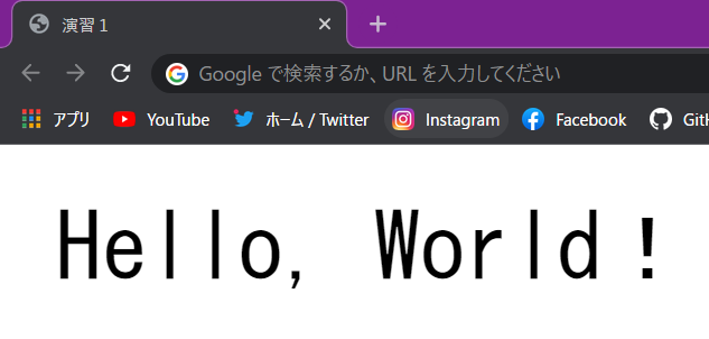
\includegraphics[height=3cm]{pic/Chap1/pic1.png}
  \end{frame}

\section*{変数とデータ型}
  \begin{frame}[plain,noframenumbering]
    \label{hensu}
    \sectionpage
  \end{frame}

  \begin{frame}{進度}
    \begin{tikzpicture}
      [every node/.style={rounded corners,inner sep=5pt, minimum width=100pt,minimum height=35pt},
      pre-subj/.style={fill=blue!20},now-subj/.style={white,fill=black!50!green},post-subj/.style={fill=black!20},overlay, remember picture]
      \node[post-subj] (a) at (0.15\textwidth,0.375\textheight){\hyperlink{programming}{プログラミング}};
      \node[now-subj,below=10pt of a] (b) {\hyperlink{hensu}{変数とデータ型}};
      \node[pre-subj,below=10pt of b] (c) {\hyperlink{enzan}{演算と演算子}};
      \node[pre-subj,below=10pt of c] (d) {\hyperlink{seigyo}{制御構文}};
      \node[pre-subj,below=10pt of d] (e) {\hyperlink{hairetsu}{配列}};
      \node[pre-subj,right=10pt of e] (f) {\hyperlink{object}{オブジェクト}};
      \node[pre-subj,above=10pt of f] (g) {\hyperlink{kansu}{関数}};
      \node[pre-subj,above=10pt of g] (h) {\hyperlink{pointa}{ポインタ}};
      \node[pre-subj,above=10pt of h] (i) {\hyperlink{objectbun}{オブジェクト構文}};
      \node[pre-subj,above=10pt of i] (j) {\hyperlink{computer}{コンピュータ基礎}};
      \node[pre-subj,right=10pt of j] (k) {\hyperlink{micom}{マイコン}};
      \node[pre-subj,below=10pt of k] (l) {\hyperlink{iot}{IoT}};
      \node[pre-subj,below=10pt of l] (m) {\hyperlink{analys}{プログラム解析}};
      \node[pre-subj,below=10pt of m] (n) {\hyperlink{readability}{コードの可読性}};
      \node[pre-subj,below=10pt of n] (o) {\hyperlink{learn}{言語の学習法}};
      \foreach \x / \y in {a/b,b/c,c/d,d/e,e/f,f/g,g/h,h/i,i/j,j/k,k/l,l/m,m/n,n/o}{
        \draw[->,>={Stealth[round]},line width=.5mm] (\x) -- (\y);
      }
    \end{tikzpicture}
  \end{frame}

  \begin{frame}{変数}{変数について}
    \begin{large}変数とは\end{large}
    \begin{itemize}
      \setlength{\itemsep}{3mm}
      \item データを入れる\structure{箱}
      \item 入れる\structure{データ}によって種類がある
      \item 箱をひとまとめにしたもの\quad\begin{large}$\triangleright$\end{large}\quad\structure{\hyperlink{hairetsu}{配列}}
    \end{itemize}
    \vfill
    \begin{large}変数の基本要素\end{large}
    \begin{itemize}
      \setlength{\itemsep}{3mm}
      \item \alert{宣言}\\
      変数を\structure{作成}すること
      \item \alert{初期化}\\
      変数の作成とともに\structure{数値を割り当てる}こと
      \item \alert{代入}\\
      変数の値を\structure{上書き}すること
    \end{itemize}
    \begin{tikzpicture}[overlay,remember picture]
      \node[at=(current page.east), anchor=east] {
        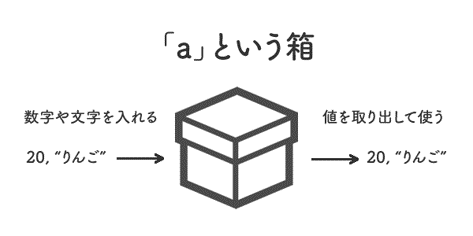
\includegraphics[height=2.4cm]{pic/Chap2/pic1.png}};
    \end{tikzpicture}
  \end{frame}

  \begin{frame}{変数}{宣言}
    \begin{itemize}
      \setlength{\itemsep}{5mm}
      \item どのような言語でも\structure{基本おなじ}
      (pythonでは宣言が暗黙)
      \item \structure{(修飾子) + 型 + 変数名}で宣言\\
      \begin{center}
        \lstinline[language=javascript]|let x;|\\
        \lstinline[language=c]|int x;|
      \end{center}
      \item 変数名は\structure{予約語}以外なら原則何でも可
    \end{itemize}
  \end{frame}

  \begin{frame}{変数}{初期化}
    \begin{itemize}
      \setlength{\itemsep}{2mm}
      \item 宣言とともに値を割り当てる\\
      (pythonでは宣言と初期化がセット)
      \item 型 + 変数名 \structure{= 初期値}で宣言 + \structure{初期化}をセットで\\
      \begin{center}
        \lstinline[language=javascript]|let x = 100;|\\
        \lstinline[language=c]|int x = 100;|
      \end{center}
      \item 静的型付けでは\structure{初期値の型}が一致している必要がある。\\
      \begin{center}
        \tikz[baseline=(T.base)]{
          \node[draw=red,shape=cross out,inner sep=2pt,outer sep=0pt] (T) {
            \lstinline[language=c]|int x = 'a';|
          };%
        }
      \end{center}
    \end{itemize}
    \begin{large}初期化をしないと...\end{large}
    \begin{center}
      ランダムに適当な値(\structure{不定値})が割り当てられる\\
      javascriptでは"\structure{undefined}"と出力される\\
      \quad\begin{large}$\blacktriangleright$\end{large}予測してない結果になる可能性がある\\
      \begin{Large}$\blacktriangledown$\end{Large}\\
      基本的に\structure{宣言}と\structure{初期化}はセットでする
    \end{center}
  \end{frame}

  \begin{frame}{変数}{代入}
    \begin{itemize}
      \setlength{\itemsep}{5mm}
      \item 変数を\structure{上書き}して内部の値を更新する
      \item 宣言後 任意の場所で 変数名 \structure{= 値}\\
      \begin{center}
        \lstinline[language=javascript]|let x = 100;|\\
        \lstinline[language=javascript]|x = 200;|
      \end{center}
      \item =は実は\structure{\hyperlink{enzan}{演算子}}
    \end{itemize}
  \end{frame}

  \begin{frame}{演習2-1:問題}{変数とデータ型}
    \label{ensyu2-1}
    \begin{Large}\lstinline[language=javascript]|let|型の変数を用いて{\color{string}Hello World}を表示させる\end{Large}
    \begin{enumerate}
      \setlength{\itemsep}{5mm}
      \item \alert{宣言}は \structure{型(今回は\lstinline[language=javascript]|let|) + 変数名(適当)}
      \item \alert{初期化}は 宣言 \structure{= 初期値}
      \item 文字列は\structure{’}か\structure{”}で囲う
      \item \lstinline[language=javascript]|document.writeln(|{\color{string}\begin{footnotesize}変数名\end{footnotesize}}\lstinline[language=javascript]|)|
      を使用して表示させよう
    \end{enumerate}
  \end{frame}

  \begin{frame}{演習2-1:解答}{変数とデータ型}
    \begin{exampleblock}{演習2-1}
      \lstinputlisting[language=javascript]{Ensyu/Ensyu2/Ensyu2-1.js}
    \end{exampleblock}
    \vspace{5mm}
    \centering
    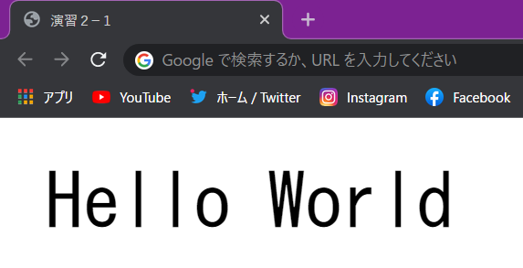
\includegraphics[height=3cm]{pic/Chap2/pic2.png}
  \end{frame}

  \begin{frame}{データ型}{データ型について}
    \begin{large}データ型とは\end{large}
    \begin{itemize}
      \setlength{\itemsep}{2mm}
      \item 変数に入る\structure{データ}を予め決めておかなければいけない\\
      $\Longrightarrow$ 予め決める言語を\structure{静的型付け}言語という
      \item 整数(\lstinline[language=c]|int|)型や 文字(\lstinline[language=c]|char|)型など多数ある
    \end{itemize}
    \vspace{2mm}
    \textreferencemark \lstinline[language=javascript]|var|型や\lstinline[language=javascript]|let|型は直接なデータ型ではない
    \begin{table}[hbtp]
      \setlength\abovecaptionskip{0pt}
      \caption{様々なデータ型}
      \label{tab:table1}
      \centering
      \footnotesize
      \begin{tabular}{lcr}
        \hline
        分類 & 名前 & 値の例\\
        \hline \hline
        論理型 & \lstinline[language=javascript]|Boolean| & True, false\\
        文字型 & \lstinline[language=c]|char| & a, b, c\\
        文字列型 & \lstinline[language=javascript]|String| & abc \\
        整数型 & \lstinline[language=c]|int| & 1, 333\\
        浮動小数点型 & \lstinline[language=c]|float|, \lstinline[language=c]|double| & 0.5, 0.0093\\
        配列型 & \lstinline[language=javascript]|Array| & [1,2,3]\\
        オブジェクト型 & \lstinline[language=javascript]|Object| & {x:1, y:2, z:3}\\
        \hline
      \end{tabular}
    \end{table}
    \centering
    \structure{言語}によってバラツキがあるので 使用したい言語で確認する
    \vspace*{3mm}
  \end{frame}

  \begin{frame}{データ型}{動的型付けについて}
    \begin{itemize}
      \setlength{\itemsep}{5mm}
      \item JavaScriptでは\structure{自動}でデータ型が割り当てられる\\
      $\Longrightarrow$ \structure{動的型付け}言語という
      \item よく使われるのは\lstinline[language=javascript]|var|と\lstinline[language=javascript]|let|の2種類
      \item \lstinline[language=javascript]|var|は\structure{宣言の重複}ができ \lstinline[language=javascript]|let|は不可
      \item \lstinline[language=javascript]|var|は後述の\structure{スコープ}が特殊なので \uuline{基本的には\lstinline[language=javascript]|let|を使用}
    \end{itemize}
  \end{frame}
  
  \begin{frame}{データ型}{データ型の使い分け}
    \begin{description}
      \setlength{\itemsep}{5mm}
      \item[\alert{サイズ}による使い分け]\mbox{}\\変数の\structure{データ型}には\alert{サイズ}がある
      \item[\alert{オーバーフロー}]\mbox{}\\サイズを超えると\structure{エラー}が起きたり\\\structure{予想しない}結果になることも
    \end{description}
    \vspace{5mm}
    \textreferencemark 使用する言語で変数のサイズを確認して使用しよう
  \end{frame}

  \begin{frame}{演習2-2:問題}{変数とデータ型}
    \begin{Large}\lstinline[language=javascript]|var|型と\lstinline[language=javascript]|let|型の違いを確認する(\alert{宣言の重複})\end{Large}\\
    \begin{enumerate}
      \setlength{\itemsep}{5mm}
      \item \lstinline[language=javascript]|var|型の変数1を\structure{宣言+初期化}する
      \item \lstinline[language=javascript]|var|型の変数1をもう一度\structure{宣言+初期化}し 表示
      \item \lstinline[language=javascript]|let|型の変数2を\structure{宣言+初期化}する
      \item \lstinline[language=javascript]|let|型の変数2をもう一度\structure{宣言+初期化}し 表示
    \end{enumerate}
    \textreferencemark 変数については\hyperlink{ensyu2-1}{演習2-1}を参照\\\lstinline[language=javascript]|document.writeln('')|を使用し 表示
  \end{frame}
  
  \begin{frame}{演習2-2:解答}{変数とデータ型}
    \begin{columns}
      \begin{column}{0.41\textwidth}
        \begin{exampleblock}{演習2-2}
          \lstinputlisting[language=javascript]{Ensyu/Ensyu2/Ensyu2-2.js}
        \end{exampleblock}
      \end{column}
      \begin{column}{0.6\textwidth}
        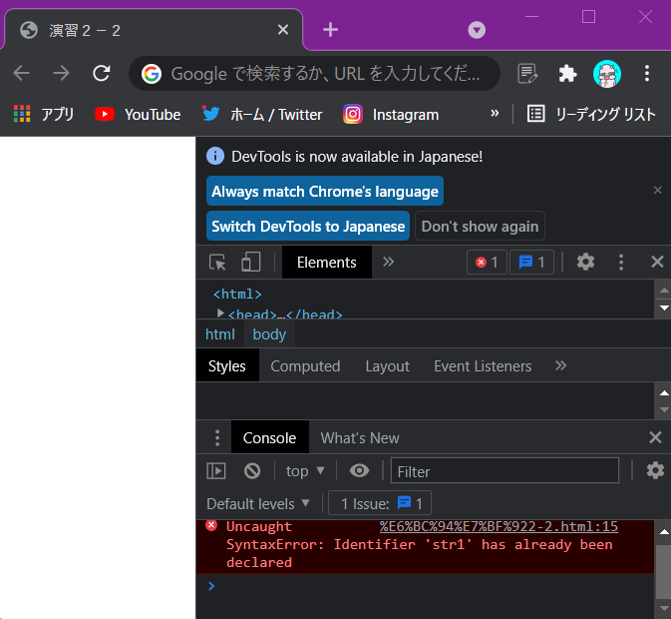
\includegraphics[width=\textwidth]{pic/Chap2/pic3.png}
      \end{column}
    \end{columns}
  \end{frame}
  
\section*{演算と演算子}
  \begin{frame}[plain,noframenumbering]
    \label{enzan}
    \sectionpage
  \end{frame}
  
  \begin{frame}{進度}
    \begin{tikzpicture}
      [every node/.style={rounded corners,inner sep=5pt, minimum width=100pt,minimum height=35pt},
      pre-subj/.style={fill=blue!20},now-subj/.style={white,fill=black!50!green},post-subj/.style={fill=black!20},overlay, remember picture]
      \node[post-subj] (a) at (0.15\textwidth,0.375\textheight){\hyperlink{programming}{プログラミング}};
      \node[post-subj,below=10pt of a] (b) {\hyperlink{hensu}{変数とデータ型}};
      \node[now-subj,below=10pt of b] (c) {\hyperlink{enzan}{演算と演算子}};
      \node[pre-subj,below=10pt of c] (d) {\hyperlink{seigyo}{制御構文}};
      \node[pre-subj,below=10pt of d] (e) {\hyperlink{hairetsu}{配列}};
      \node[pre-subj,right=10pt of e] (f) {\hyperlink{object}{オブジェクト}};
      \node[pre-subj,above=10pt of f] (g) {\hyperlink{kansu}{関数}};
      \node[pre-subj,above=10pt of g] (h) {\hyperlink{pointa}{ポインタ}};
      \node[pre-subj,above=10pt of h] (i) {\hyperlink{objectbun}{オブジェクト構文}};
      \node[pre-subj,above=10pt of i] (j) {\hyperlink{computer}{コンピュータ基礎}};
      \node[pre-subj,right=10pt of j] (k) {\hyperlink{micom}{マイコン}};
      \node[pre-subj,below=10pt of k] (l) {\hyperlink{iot}{IoT}};
      \node[pre-subj,below=10pt of l] (m) {\hyperlink{analys}{プログラム解析}};
      \node[pre-subj,below=10pt of m] (n) {\hyperlink{readability}{コードの可読性}};
      \node[pre-subj,below=10pt of n] (o) {\hyperlink{learn}{言語の学習法}};
      \foreach \x / \y in {a/b,b/c,c/d,d/e,e/f,f/g,g/h,h/i,i/j,j/k,k/l,l/m,m/n,n/o}{
        \draw[->,>={Stealth[round]},line width=.5mm] (\x) -- (\y);
      }
    \end{tikzpicture}
  \end{frame}

\section*{制御構文}
  \begin{frame}[plain,noframenumbering]
    \label{seigyo}
    \sectionpage
  \end{frame}
  
  \begin{frame}{進度}
    \begin{tikzpicture}
      [every node/.style={rounded corners,inner sep=5pt, minimum width=100pt,minimum height=35pt},
      pre-subj/.style={fill=blue!20},now-subj/.style={white,fill=black!50!green},post-subj/.style={fill=black!20},overlay, remember picture]
      \node[post-subj] (a) at (0.15\textwidth,0.375\textheight){\hyperlink{programming}{プログラミング}};
      \node[post-subj,below=10pt of a] (b) {\hyperlink{hensu}{変数とデータ型}};
      \node[post-subj,below=10pt of b] (c) {\hyperlink{enzan}{演算と演算子}};
      \node[now-subj,below=10pt of c] (d) {\hyperlink{seigyo}{制御構文}};
      \node[pre-subj,below=10pt of d] (e) {\hyperlink{hairetsu}{配列}};
      \node[pre-subj,right=10pt of e] (f) {\hyperlink{object}{オブジェクト}};
      \node[pre-subj,above=10pt of f] (g) {\hyperlink{kansu}{関数}};
      \node[pre-subj,above=10pt of g] (h) {\hyperlink{pointa}{ポインタ}};
      \node[pre-subj,above=10pt of h] (i) {\hyperlink{objectbun}{オブジェクト構文}};
      \node[pre-subj,above=10pt of i] (j) {\hyperlink{computer}{コンピュータ基礎}};
      \node[pre-subj,right=10pt of j] (k) {\hyperlink{micom}{マイコン}};
      \node[pre-subj,below=10pt of k] (l) {\hyperlink{iot}{IoT}};
      \node[pre-subj,below=10pt of l] (m) {\hyperlink{analys}{プログラム解析}};
      \node[pre-subj,below=10pt of m] (n) {\hyperlink{readability}{コードの可読性}};
      \node[pre-subj,below=10pt of n] (o) {\hyperlink{learn}{言語の学習法}};
      \foreach \x / \y in {a/b,b/c,c/d,d/e,e/f,f/g,g/h,h/i,i/j,j/k,k/l,l/m,m/n,n/o}{
        \draw[->,>={Stealth[round]},line width=.5mm] (\x) -- (\y);
      }
    \end{tikzpicture}
  \end{frame}

\section*{配列}
  \begin{frame}[plain,noframenumbering]
    \label{hairetsu}
    \sectionpage
  \end{frame}
  
  \begin{frame}{進度}
    \begin{tikzpicture}
      [every node/.style={rounded corners,inner sep=5pt, minimum width=100pt,minimum height=35pt},
      pre-subj/.style={fill=blue!20},now-subj/.style={white,fill=black!50!green},post-subj/.style={fill=black!20},overlay, remember picture]
      \node[post-subj] (a) at (0.15\textwidth,0.375\textheight){\hyperlink{programming}{プログラミング}};
      \node[post-subj,below=10pt of a] (b) {\hyperlink{hensu}{変数とデータ型}};
      \node[post-subj,below=10pt of b] (c) {\hyperlink{enzan}{演算と演算子}};
      \node[post-subj,below=10pt of c] (d) {\hyperlink{seigyo}{制御構文}};
      \node[now-subj,below=10pt of d] (e) {\hyperlink{hairetsu}{配列}};
      \node[pre-subj,right=10pt of e] (f) {\hyperlink{object}{オブジェクト}};
      \node[pre-subj,above=10pt of f] (g) {\hyperlink{kansu}{関数}};
      \node[pre-subj,above=10pt of g] (h) {\hyperlink{pointa}{ポインタ}};
      \node[pre-subj,above=10pt of h] (i) {\hyperlink{objectbun}{オブジェクト構文}};
      \node[pre-subj,above=10pt of i] (j) {\hyperlink{computer}{コンピュータ基礎}};
      \node[pre-subj,right=10pt of j] (k) {\hyperlink{micom}{マイコン}};
      \node[pre-subj,below=10pt of k] (l) {\hyperlink{iot}{IoT}};
      \node[pre-subj,below=10pt of l] (m) {\hyperlink{analys}{プログラム解析}};
      \node[pre-subj,below=10pt of m] (n) {\hyperlink{readability}{コードの可読性}};
      \node[pre-subj,below=10pt of n] (o) {\hyperlink{learn}{言語の学習法}};
      \foreach \x / \y in {a/b,b/c,c/d,d/e,e/f,f/g,g/h,h/i,i/j,j/k,k/l,l/m,m/n,n/o}{
        \draw[->,>={Stealth[round]},line width=.5mm] (\x) -- (\y);
      }
    \end{tikzpicture}
  \end{frame}

\section*{オブジェクト}
  \begin{frame}[plain,noframenumbering]
    \label{object}
    \sectionpage
  \end{frame}
  
  \begin{frame}{進度}
    \begin{tikzpicture}
      [every node/.style={rounded corners,inner sep=5pt, minimum width=100pt,minimum height=35pt},
      pre-subj/.style={fill=blue!20},now-subj/.style={white,fill=black!50!green},post-subj/.style={fill=black!20},overlay, remember picture]
      \node[post-subj] (a) at (0.15\textwidth,0.375\textheight){\hyperlink{programming}{プログラミング}};
      \node[post-subj,below=10pt of a] (b) {\hyperlink{hensu}{変数とデータ型}};
      \node[post-subj,below=10pt of b] (c) {\hyperlink{enzan}{演算と演算子}};
      \node[post-subj,below=10pt of c] (d) {\hyperlink{seigyo}{制御構文}};
      \node[post-subj,below=10pt of d] (e) {\hyperlink{hairetsu}{配列}};
      \node[now-subj,right=10pt of e] (f) {\hyperlink{object}{オブジェクト}};
      \node[pre-subj,above=10pt of f] (g) {\hyperlink{kansu}{関数}};
      \node[pre-subj,above=10pt of g] (h) {\hyperlink{pointa}{ポインタ}};
      \node[pre-subj,above=10pt of h] (i) {\hyperlink{objectbun}{オブジェクト構文}};
      \node[pre-subj,above=10pt of i] (j) {\hyperlink{computer}{コンピュータ基礎}};
      \node[pre-subj,right=10pt of j] (k) {\hyperlink{micom}{マイコン}};
      \node[pre-subj,below=10pt of k] (l) {\hyperlink{iot}{IoT}};
      \node[pre-subj,below=10pt of l] (m) {\hyperlink{analys}{プログラム解析}};
      \node[pre-subj,below=10pt of m] (n) {\hyperlink{readability}{コードの可読性}};
      \node[pre-subj,below=10pt of n] (o) {\hyperlink{learn}{言語の学習法}};
      \foreach \x / \y in {a/b,b/c,c/d,d/e,e/f,f/g,g/h,h/i,i/j,j/k,k/l,l/m,m/n,n/o}{
        \draw[->,>={Stealth[round]},line width=.5mm] (\x) -- (\y);
      }
    \end{tikzpicture}
  \end{frame}

\section*{関数}
  \begin{frame}[plain,noframenumbering]
    \label{kansu}
    \sectionpage
  \end{frame}
  
  \begin{frame}{進度}
    \begin{tikzpicture}
      [every node/.style={rounded corners,inner sep=5pt, minimum width=100pt,minimum height=35pt},
      pre-subj/.style={fill=blue!20},now-subj/.style={white,fill=black!50!green},post-subj/.style={fill=black!20},overlay, remember picture]
      \node[post-subj] (a) at (0.15\textwidth,0.375\textheight){\hyperlink{programming}{プログラミング}};
      \node[post-subj,below=10pt of a] (b) {\hyperlink{hensu}{変数とデータ型}};
      \node[post-subj,below=10pt of b] (c) {\hyperlink{enzan}{演算と演算子}};
      \node[post-subj,below=10pt of c] (d) {\hyperlink{seigyo}{制御構文}};
      \node[post-subj,below=10pt of d] (e) {\hyperlink{hairetsu}{配列}};
      \node[post-subj,right=10pt of e] (f) {\hyperlink{object}{オブジェクト}};
      \node[now-subj,above=10pt of f] (g) {\hyperlink{kansu}{関数}};
      \node[pre-subj,above=10pt of g] (h) {\hyperlink{pointa}{ポインタ}};
      \node[pre-subj,above=10pt of h] (i) {\hyperlink{objectbun}{オブジェクト構文}};
      \node[pre-subj,above=10pt of i] (j) {\hyperlink{computer}{コンピュータ基礎}};
      \node[pre-subj,right=10pt of j] (k) {\hyperlink{micom}{マイコン}};
      \node[pre-subj,below=10pt of k] (l) {\hyperlink{iot}{IoT}};
      \node[pre-subj,below=10pt of l] (m) {\hyperlink{analys}{プログラム解析}};
      \node[pre-subj,below=10pt of m] (n) {\hyperlink{readability}{コードの可読性}};
      \node[pre-subj,below=10pt of n] (o) {\hyperlink{learn}{言語の学習法}};
      \foreach \x / \y in {a/b,b/c,c/d,d/e,e/f,f/g,g/h,h/i,i/j,j/k,k/l,l/m,m/n,n/o}{
        \draw[->,>={Stealth[round]},line width=.5mm] (\x) -- (\y);
      }
    \end{tikzpicture}
  \end{frame}

\section*{ポインタ}
  \begin{frame}[plain,noframenumbering]
    \label{pointa}
    \sectionpage
  \end{frame}

  \begin{frame}{進度}
    \begin{tikzpicture}
      [every node/.style={rounded corners,inner sep=5pt, minimum width=100pt,minimum height=35pt},
      pre-subj/.style={fill=blue!20},now-subj/.style={white,fill=black!50!green},post-subj/.style={fill=black!20},overlay, remember picture]
      \node[post-subj] (a) at (0.15\textwidth,0.375\textheight){\hyperlink{programming}{プログラミング}};
      \node[post-subj,below=10pt of a] (b) {\hyperlink{hensu}{変数とデータ型}};
      \node[post-subj,below=10pt of b] (c) {\hyperlink{enzan}{演算と演算子}};
      \node[post-subj,below=10pt of c] (d) {\hyperlink{seigyo}{制御構文}};
      \node[post-subj,below=10pt of d] (e) {\hyperlink{hairetsu}{配列}};
      \node[post-subj,right=10pt of e] (f) {\hyperlink{object}{オブジェクト}};
      \node[post-subj,above=10pt of f] (g) {\hyperlink{kansu}{関数}};
      \node[now-subj,above=10pt of g] (h) {\hyperlink{pointa}{ポインタ}};
      \node[pre-subj,above=10pt of h] (i) {\hyperlink{objectbun}{オブジェクト構文}};
      \node[pre-subj,above=10pt of i] (j) {\hyperlink{computer}{コンピュータ基礎}};
      \node[pre-subj,right=10pt of j] (k) {\hyperlink{micom}{マイコン}};
      \node[pre-subj,below=10pt of k] (l) {\hyperlink{iot}{IoT}};
      \node[pre-subj,below=10pt of l] (m) {\hyperlink{analys}{プログラム解析}};
      \node[pre-subj,below=10pt of m] (n) {\hyperlink{readability}{コードの可読性}};
      \node[pre-subj,below=10pt of n] (o) {\hyperlink{learn}{言語の学習法}};
      \foreach \x / \y in {a/b,b/c,c/d,d/e,e/f,f/g,g/h,h/i,i/j,j/k,k/l,l/m,m/n,n/o}{
        \draw[->,>={Stealth[round]},line width=.5mm] (\x) -- (\y);
      }
    \end{tikzpicture}
  \end{frame}
  
\section*{オブジェクト指向構文}
  \begin{frame}[plain,noframenumbering]
    \label{objectbun}
    \sectionpage
  \end{frame}

  \begin{frame}{進度}
    \begin{tikzpicture}
      [every node/.style={rounded corners,inner sep=5pt, minimum width=100pt,minimum height=35pt},
      pre-subj/.style={fill=blue!20},now-subj/.style={white,fill=black!50!green},post-subj/.style={fill=black!20},overlay, remember picture]
      \node[post-subj] (a) at (0.15\textwidth,0.375\textheight){\hyperlink{programming}{プログラミング}};
      \node[post-subj,below=10pt of a] (b) {\hyperlink{hensu}{変数とデータ型}};
      \node[post-subj,below=10pt of b] (c) {\hyperlink{enzan}{演算と演算子}};
      \node[post-subj,below=10pt of c] (d) {\hyperlink{seigyo}{制御構文}};
      \node[post-subj,below=10pt of d] (e) {\hyperlink{hairetsu}{配列}};
      \node[post-subj,right=10pt of e] (f) {\hyperlink{object}{オブジェクト}};
      \node[post-subj,above=10pt of f] (g) {\hyperlink{kansu}{関数}};
      \node[post-subj,above=10pt of g] (h) {\hyperlink{pointa}{ポインタ}};
      \node[now-subj,above=10pt of h] (i) {\hyperlink{objectbun}{オブジェクト構文}};
      \node[pre-subj,above=10pt of i] (j) {\hyperlink{computer}{コンピュータ基礎}};
      \node[pre-subj,right=10pt of j] (k) {\hyperlink{micom}{マイコン}};
      \node[pre-subj,below=10pt of k] (l) {\hyperlink{iot}{IoT}};
      \node[pre-subj,below=10pt of l] (m) {\hyperlink{analys}{プログラム解析}};
      \node[pre-subj,below=10pt of m] (n) {\hyperlink{readability}{コードの可読性}};
      \node[pre-subj,below=10pt of n] (o) {\hyperlink{learn}{言語の学習法}};
      \foreach \x / \y in {a/b,b/c,c/d,d/e,e/f,f/g,g/h,h/i,i/j,j/k,k/l,l/m,m/n,n/o}{
        \draw[->,>={Stealth[round]},line width=.5mm] (\x) -- (\y);
      }
    \end{tikzpicture}
  \end{frame}

\section*{コンピュータ基礎}
  \begin{frame}[plain,noframenumbering]
    \label{computer}
    \sectionpage
  \end{frame}

  \begin{frame}{進度}
    \begin{tikzpicture}
      [every node/.style={rounded corners,inner sep=5pt, minimum width=100pt,minimum height=35pt},
      pre-subj/.style={fill=blue!20},now-subj/.style={white,fill=black!50!green},post-subj/.style={fill=black!20},overlay, remember picture]
      \node[post-subj] (a) at (0.15\textwidth,0.375\textheight){\hyperlink{programming}{プログラミング}};
      \node[post-subj,below=10pt of a] (b) {\hyperlink{hensu}{変数とデータ型}};
      \node[post-subj,below=10pt of b] (c) {\hyperlink{enzan}{演算と演算子}};
      \node[post-subj,below=10pt of c] (d) {\hyperlink{seigyo}{制御構文}};
      \node[post-subj,below=10pt of d] (e) {\hyperlink{hairetsu}{配列}};
      \node[post-subj,right=10pt of e] (f) {\hyperlink{object}{オブジェクト}};
      \node[post-subj,above=10pt of f] (g) {\hyperlink{kansu}{関数}};
      \node[post-subj,above=10pt of g] (h) {\hyperlink{pointa}{ポインタ}};
      \node[post-subj,above=10pt of h] (i) {\hyperlink{objectbun}{オブジェクト構文}};
      \node[now-subj,above=10pt of i] (j) {\hyperlink{computer}{コンピュータ基礎}};
      \node[pre-subj,right=10pt of j] (k) {\hyperlink{micom}{マイコン}};
      \node[pre-subj,below=10pt of k] (l) {\hyperlink{iot}{IoT}};
      \node[pre-subj,below=10pt of l] (m) {\hyperlink{analys}{プログラム解析}};
      \node[pre-subj,below=10pt of m] (n) {\hyperlink{readability}{コードの可読性}};
      \node[pre-subj,below=10pt of n] (o) {\hyperlink{learn}{言語の学習法}};
      \foreach \x / \y in {a/b,b/c,c/d,d/e,e/f,f/g,g/h,h/i,i/j,j/k,k/l,l/m,m/n,n/o}{
        \draw[->,>={Stealth[round]},line width=.5mm] (\x) -- (\y);
      }
    \end{tikzpicture}
  \end{frame}

\section*{マイコン}
  \begin{frame}[plain,noframenumbering]
    \label{micom}
    \sectionpage
  \end{frame}
  
  \begin{frame}{進度}
    \begin{tikzpicture}
      [every node/.style={rounded corners,inner sep=5pt, minimum width=100pt,minimum height=35pt},
      pre-subj/.style={fill=blue!20},now-subj/.style={white,fill=black!50!green},post-subj/.style={fill=black!20},overlay, remember picture]
      \node[post-subj] (a) at (0.15\textwidth,0.375\textheight){\hyperlink{programming}{プログラミング}};
      \node[post-subj,below=10pt of a] (b) {\hyperlink{hensu}{変数とデータ型}};
      \node[post-subj,below=10pt of b] (c) {\hyperlink{enzan}{演算と演算子}};
      \node[post-subj,below=10pt of c] (d) {\hyperlink{seigyo}{制御構文}};
      \node[post-subj,below=10pt of d] (e) {\hyperlink{hairetsu}{配列}};
      \node[post-subj,right=10pt of e] (f) {\hyperlink{object}{オブジェクト}};
      \node[post-subj,above=10pt of f] (g) {\hyperlink{kansu}{関数}};
      \node[post-subj,above=10pt of g] (h) {\hyperlink{pointa}{ポインタ}};
      \node[post-subj,above=10pt of h] (i) {\hyperlink{objectbun}{オブジェクト構文}};
      \node[post-subj,above=10pt of i] (j) {\hyperlink{computer}{コンピュータ基礎}};
      \node[now-subj,right=10pt of j] (k) {\hyperlink{micom}{マイコン}};
      \node[pre-subj,below=10pt of k] (l) {\hyperlink{iot}{IoT}};
      \node[pre-subj,below=10pt of l] (m) {\hyperlink{analys}{プログラム解析}};
      \node[pre-subj,below=10pt of m] (n) {\hyperlink{readability}{コードの可読性}};
      \node[pre-subj,below=10pt of n] (o) {\hyperlink{learn}{言語の学習法}};
      \foreach \x / \y in {a/b,b/c,c/d,d/e,e/f,f/g,g/h,h/i,i/j,j/k,k/l,l/m,m/n,n/o}{
        \draw[->,>={Stealth[round]},line width=.5mm] (\x) -- (\y);
      }
    \end{tikzpicture}
  \end{frame}

\section*{IoT}
  \begin{frame}[plain,noframenumbering]
    \label{iot}
    \sectionpage
  \end{frame}

  \begin{frame}{進度}
    \begin{tikzpicture}
      [every node/.style={rounded corners,inner sep=5pt, minimum width=100pt,minimum height=35pt},
      pre-subj/.style={fill=blue!20},now-subj/.style={white,fill=black!50!green},post-subj/.style={fill=black!20},overlay, remember picture]
      \node[post-subj] (a) at (0.15\textwidth,0.375\textheight){\hyperlink{programming}{プログラミング}};
      \node[post-subj,below=10pt of a] (b) {\hyperlink{hensu}{変数とデータ型}};
      \node[post-subj,below=10pt of b] (c) {\hyperlink{enzan}{演算と演算子}};
      \node[post-subj,below=10pt of c] (d) {\hyperlink{seigyo}{制御構文}};
      \node[post-subj,below=10pt of d] (e) {\hyperlink{hairetsu}{配列}};
      \node[post-subj,right=10pt of e] (f) {\hyperlink{object}{オブジェクト}};
      \node[post-subj,above=10pt of f] (g) {\hyperlink{kansu}{関数}};
      \node[post-subj,above=10pt of g] (h) {\hyperlink{pointa}{ポインタ}};
      \node[post-subj,above=10pt of h] (i) {\hyperlink{objectbun}{オブジェクト構文}};
      \node[post-subj,above=10pt of i] (j) {\hyperlink{computer}{コンピュータ基礎}};
      \node[post-subj,right=10pt of j] (k) {\hyperlink{micom}{マイコン}};
      \node[now-subj,below=10pt of k] (l) {\hyperlink{iot}{IoT}};
      \node[pre-subj,below=10pt of l] (m) {\hyperlink{analys}{プログラム解析}};
      \node[pre-subj,below=10pt of m] (n) {\hyperlink{readability}{コードの可読性}};
      \node[pre-subj,below=10pt of n] (o) {\hyperlink{learn}{言語の学習法}};
      \foreach \x / \y in {a/b,b/c,c/d,d/e,e/f,f/g,g/h,h/i,i/j,j/k,k/l,l/m,m/n,n/o}{
        \draw[->,>={Stealth[round]},line width=.5mm] (\x) -- (\y);
      }
    \end{tikzpicture}
  \end{frame}

\section*{プログラム解析}
  \begin{frame}[plain,noframenumbering]
    \label{analys}
    \sectionpage
  \end{frame}

  \begin{frame}{進度}
    \begin{tikzpicture}
      [every node/.style={rounded corners,inner sep=5pt, minimum width=100pt,minimum height=35pt},
      pre-subj/.style={fill=blue!20},now-subj/.style={white,fill=black!50!green},post-subj/.style={fill=black!20},overlay, remember picture]
      \node[post-subj] (a) at (0.15\textwidth,0.375\textheight){\hyperlink{programming}{プログラミング}};
      \node[post-subj,below=10pt of a] (b) {\hyperlink{hensu}{変数とデータ型}};
      \node[post-subj,below=10pt of b] (c) {\hyperlink{enzan}{演算と演算子}};
      \node[post-subj,below=10pt of c] (d) {\hyperlink{seigyo}{制御構文}};
      \node[post-subj,below=10pt of d] (e) {\hyperlink{hairetsu}{配列}};
      \node[post-subj,right=10pt of e] (f) {\hyperlink{object}{オブジェクト}};
      \node[post-subj,above=10pt of f] (g) {\hyperlink{kansu}{関数}};
      \node[post-subj,above=10pt of g] (h) {\hyperlink{pointa}{ポインタ}};
      \node[post-subj,above=10pt of h] (i) {\hyperlink{objectbun}{オブジェクト構文}};
      \node[post-subj,above=10pt of i] (j) {\hyperlink{computer}{コンピュータ基礎}};
      \node[post-subj,right=10pt of j] (k) {\hyperlink{micom}{マイコン}};
      \node[post-subj,below=10pt of k] (l) {\hyperlink{iot}{IoT}};
      \node[now-subj,below=10pt of l] (m) {\hyperlink{analys}{プログラム解析}};
      \node[pre-subj,below=10pt of m] (n) {\hyperlink{readability}{コードの可読性}};
      \node[pre-subj,below=10pt of n] (o) {\hyperlink{learn}{言語の学習法}};
      \foreach \x / \y in {a/b,b/c,c/d,d/e,e/f,f/g,g/h,h/i,i/j,j/k,k/l,l/m,m/n,n/o}{
        \draw[->,>={Stealth[round]},line width=.5mm] (\x) -- (\y);
      }
    \end{tikzpicture}
  \end{frame}

\section*{コードの可読性}
  \begin{frame}[plain,noframenumbering]
    \label{readability}
    \sectionpage
  \end{frame}

  \begin{frame}{進度}
    \begin{tikzpicture}
      [every node/.style={rounded corners,inner sep=5pt, minimum width=100pt,minimum height=35pt},
      pre-subj/.style={fill=blue!20},now-subj/.style={white,fill=black!50!green},post-subj/.style={fill=black!20},overlay, remember picture]
      \node[post-subj] (a) at (0.15\textwidth,0.375\textheight){\hyperlink{programming}{プログラミング}};
      \node[post-subj,below=10pt of a] (b) {\hyperlink{hensu}{変数とデータ型}};
      \node[post-subj,below=10pt of b] (c) {\hyperlink{enzan}{演算と演算子}};
      \node[post-subj,below=10pt of c] (d) {\hyperlink{seigyo}{制御構文}};
      \node[post-subj,below=10pt of d] (e) {\hyperlink{hairetsu}{配列}};
      \node[post-subj,right=10pt of e] (f) {\hyperlink{object}{オブジェクト}};
      \node[post-subj,above=10pt of f] (g) {\hyperlink{kansu}{関数}};
      \node[post-subj,above=10pt of g] (h) {\hyperlink{pointa}{ポインタ}};
      \node[post-subj,above=10pt of h] (i) {\hyperlink{objectbun}{オブジェクト構文}};
      \node[post-subj,above=10pt of i] (j) {\hyperlink{computer}{コンピュータ基礎}};
      \node[post-subj,right=10pt of j] (k) {\hyperlink{micom}{マイコン}};
      \node[post-subj,below=10pt of k] (l) {\hyperlink{iot}{IoT}};
      \node[post-subj,below=10pt of l] (m) {\hyperlink{analys}{プログラム解析}};
      \node[now-subj,below=10pt of m] (n) {\hyperlink{readability}{コードの可読性}};
      \node[pre-subj,below=10pt of n] (o) {\hyperlink{learn}{言語の学習法}};
      \foreach \x / \y in {a/b,b/c,c/d,d/e,e/f,f/g,g/h,h/i,i/j,j/k,k/l,l/m,m/n,n/o}{
        \draw[->,>={Stealth[round]},line width=.5mm] (\x) -- (\y);
      }
    \end{tikzpicture}
  \end{frame}

\section*{言語の学習法}
  \begin{frame}[plain,noframenumbering]
    \label{learn}
    \sectionpage
  \end{frame}
  
  \begin{frame}{進度}
    \begin{tikzpicture}
      [every node/.style={rounded corners,inner sep=5pt, minimum width=100pt,minimum height=35pt},
      pre-subj/.style={fill=blue!20},now-subj/.style={white,fill=black!50!green},post-subj/.style={fill=black!20},overlay, remember picture]
      \node[post-subj] (a) at (0.15\textwidth,0.375\textheight){\hyperlink{programming}{プログラミング}};
      \node[post-subj,below=10pt of a] (b) {\hyperlink{hensu}{変数とデータ型}};
      \node[post-subj,below=10pt of b] (c) {\hyperlink{enzan}{演算と演算子}};
      \node[post-subj,below=10pt of c] (d) {\hyperlink{seigyo}{制御構文}};
      \node[post-subj,below=10pt of d] (e) {\hyperlink{hairetsu}{配列}};
      \node[post-subj,right=10pt of e] (f) {\hyperlink{object}{オブジェクト}};
      \node[post-subj,above=10pt of f] (g) {\hyperlink{kansu}{関数}};
      \node[post-subj,above=10pt of g] (h) {\hyperlink{pointa}{ポインタ}};
      \node[post-subj,above=10pt of h] (i) {\hyperlink{objectbun}{オブジェクト構文}};
      \node[post-subj,above=10pt of i] (j) {\hyperlink{computer}{コンピュータ基礎}};
      \node[post-subj,right=10pt of j] (k) {\hyperlink{micom}{マイコン}};
      \node[post-subj,below=10pt of k] (l) {\hyperlink{iot}{IoT}};
      \node[post-subj,below=10pt of l] (m) {\hyperlink{analys}{プログラム解析}};
      \node[post-subj,below=10pt of m] (n) {\hyperlink{readability}{コードの可読性}};
      \node[now-subj,below=10pt of n] (o) {\hyperlink{learn}{言語の学習法}};
      \foreach \x / \y in {a/b,b/c,c/d,d/e,e/f,f/g,g/h,h/i,i/j,j/k,k/l,l/m,m/n,n/o}{
        \draw[->,>={Stealth[round]},line width=.5mm] (\x) -- (\y);
      }
    \end{tikzpicture}
  \end{frame}

\section*{問題解決能力}
  \begin{frame}[plain,noframenumbering]
    \sectionpage
  \end{frame}

\end{document}